\section{Green‐Phase Vehicle Flow}
\label{sec:Results_GreenPhaseFlow}

The per-cycle vehicle flow for demand levels ranging from $69$ to $3462~\unit{\veh\per\hour}$ across \acp{mpr} is summarized in Table~\vref{tab:GreenPhaseFlow}. \enquote{Standard} ($0\%$) denotes no \ac{glosa}, and \enquote{Baseline} denotes \ac{flow-glosa}. Figure~\vref{fig:combined_flow} visualise the curves for HBEFA4 and PHEMlight5 at $2077$, $2769$ and $3462~\unit{\veh\per\hour}$. At low to moderate demand ($69$--$692~\unit{\veh\per\hour}$), both \ac{eco-glosa} and \ac{flow-glosa} remain within $\pm0.04\unit{\veh\per\hour}$ of the Standard across the full \ac{mpr} range. This implies that speed advisories, regardless of whether they are emission- or flow-optimized, do not significantly impact green-phase capacity in the presence of low traffic densities. Beyond the $2077~\unit{\veh\per\hour}$ breakpoint, the throughput of the \ac{eco-glosa} controller declines sharply. For instance, at a demand of $2769~\unit{\veh\per\hour}$ under the PHEMlight5 model, the flow drops from $46.03$ vehicles at Standard to $35.90$ vehicles at $90\%$ \ac{mpr}, a reduction of $22\%$. A similar decline occurs at $3462~\unit{\veh\per\hour}$ with the HBEFA4 model, where throughput falls from $49.03$ to $37.27$ vehicles at full \ac{mpr}. This provides clear evidence of queue formation and spill‐back occurring within a single green phase. In contrast, the \ac{flow-glosa} baseline curves exhibit modest throughput gains at high penetration under heavy demand, increasing flow above the Standard by up to $17.5\%$ at $3462~\unit{\veh\per\hour}$. The findings of this study confirm, that \ac{eco-glosa} does not affect the flow at low densities, but its emission-driven advisories incur substantial capacity penalties during periods of high demand. Conversely, \ac{flow-glosa} not only maintains, but also improves green-phase capacity at full penetration.

\begin{figure}[htb]
  \centering
  % first two subfigures
  \begin{subfigure}[t]{0.98\textwidth}
    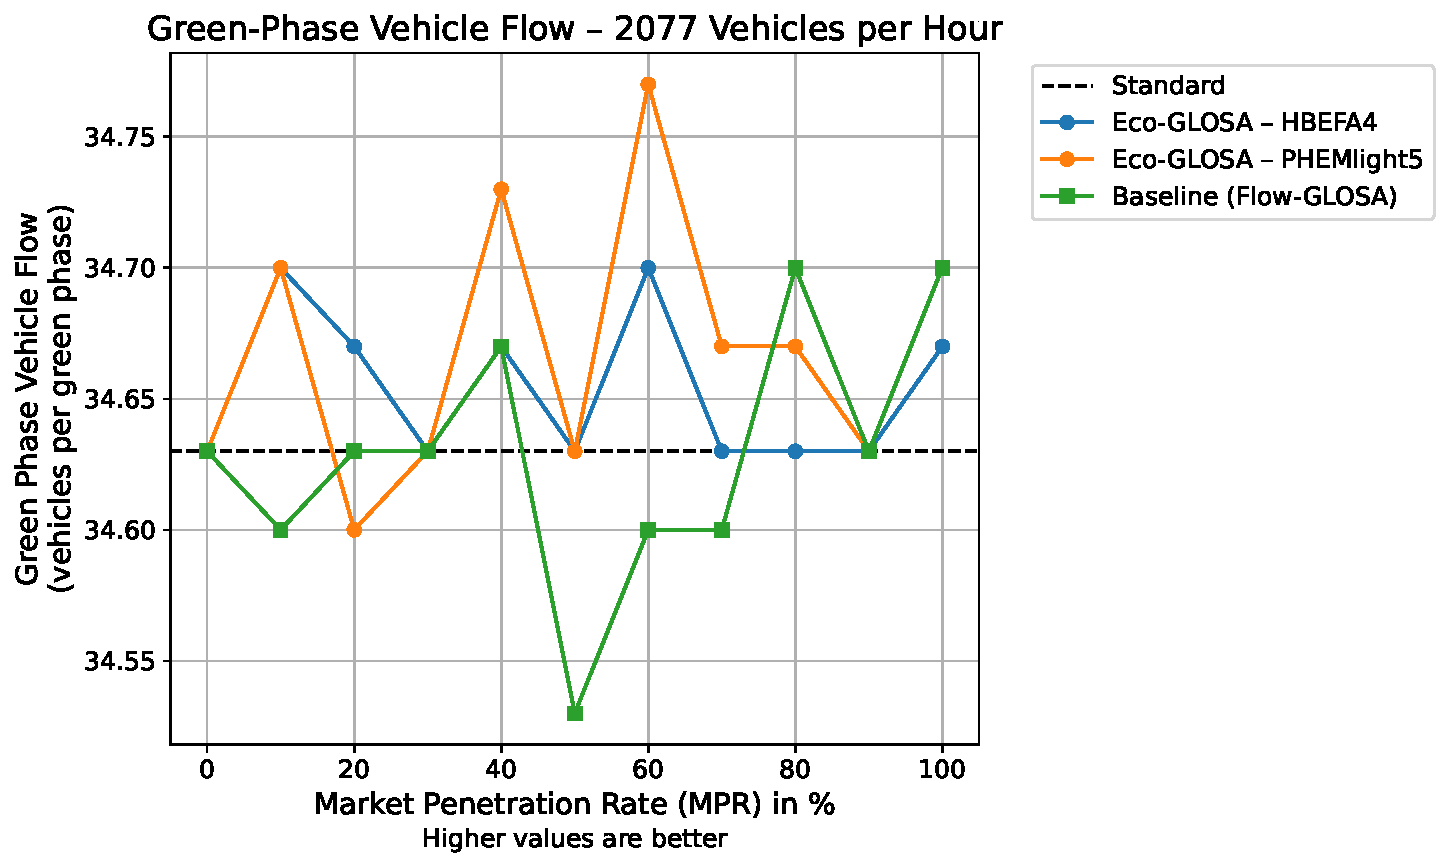
\includegraphics[width=\textwidth]{data/img/GreenPhaseVehicleFlow/GreenPhaseVehicleFlow_Cars1500.pdf}
    \caption{$2077~\unit{\veh\per\hour}$}
    \label{fig:flow_2077}
  \end{subfigure}\hfill
  \begin{subfigure}[t]{0.98\textwidth}
    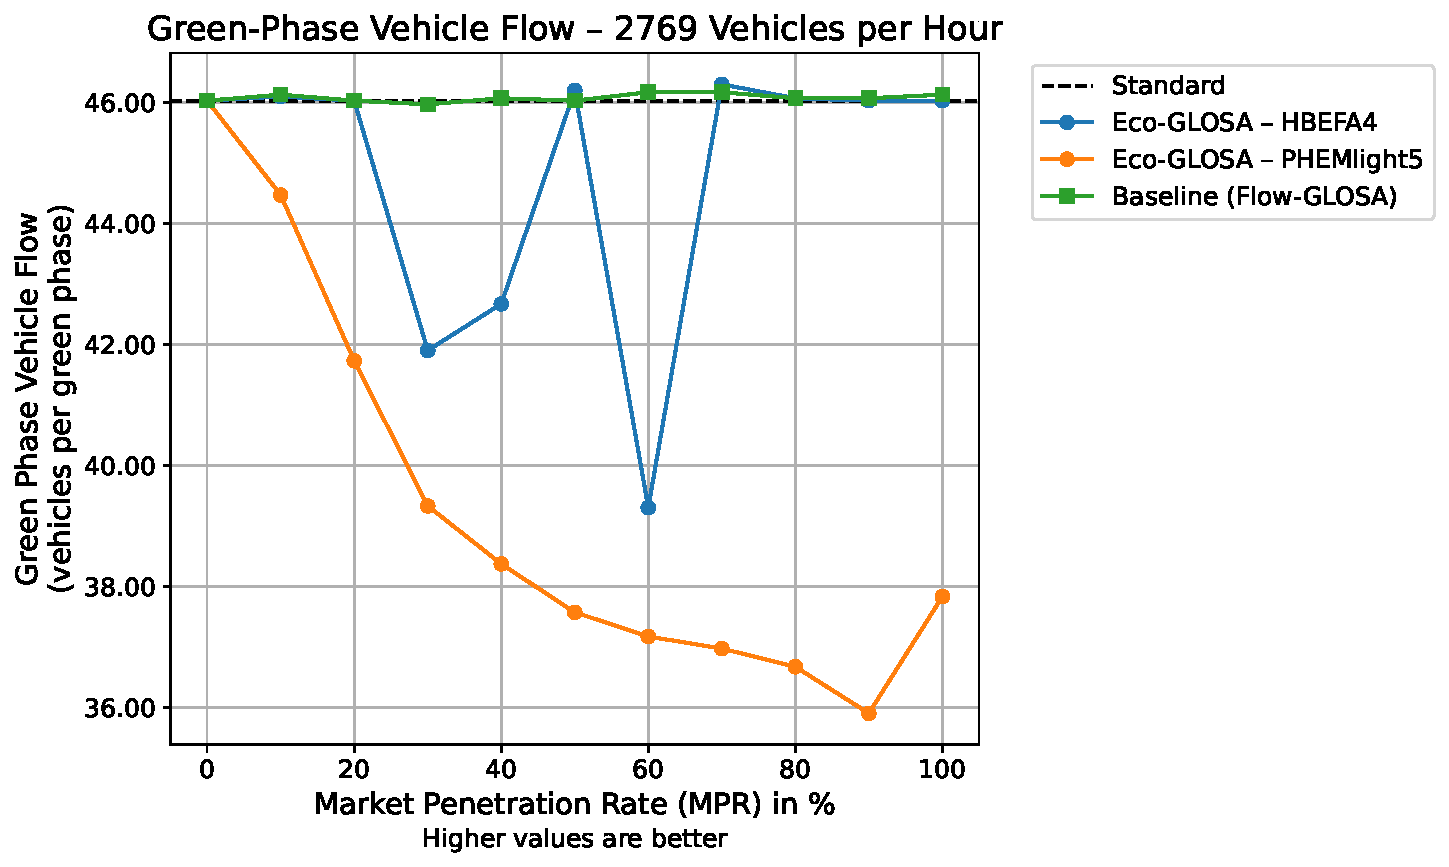
\includegraphics[width=\textwidth]{data/img/GreenPhaseVehicleFlow/GreenPhaseVehicleFlow_Cars2000.pdf}
    \caption{$2769~\unit{\veh\per\hour}$}
    \label{fig:flow_2769}
  \end{subfigure}
  \caption[Green–phase vehicle flow vs. \ac{mpr} at $2077$ and $2769~\unit{\veh\per\hour}$]{%
    Green–phase vehicle flow as a function of \ac{mpr} for two high‐demand scenarios. Each plot compares the Standard (no \ac{glosa}), \ac{eco-glosa} (HBEFA4 and PHEMlight5), and \ac{flow-glosa} controllers at $2077$ and $2769~\unit{\veh\per\hour}$.%
  }
  \label{fig:combined_flow}
\end{figure}

\begin{figure}[htb]\ContinuedFloat
  \centering
  % remaining subfigure on next page
  \begin{subfigure}[t]{0.98\textwidth}
    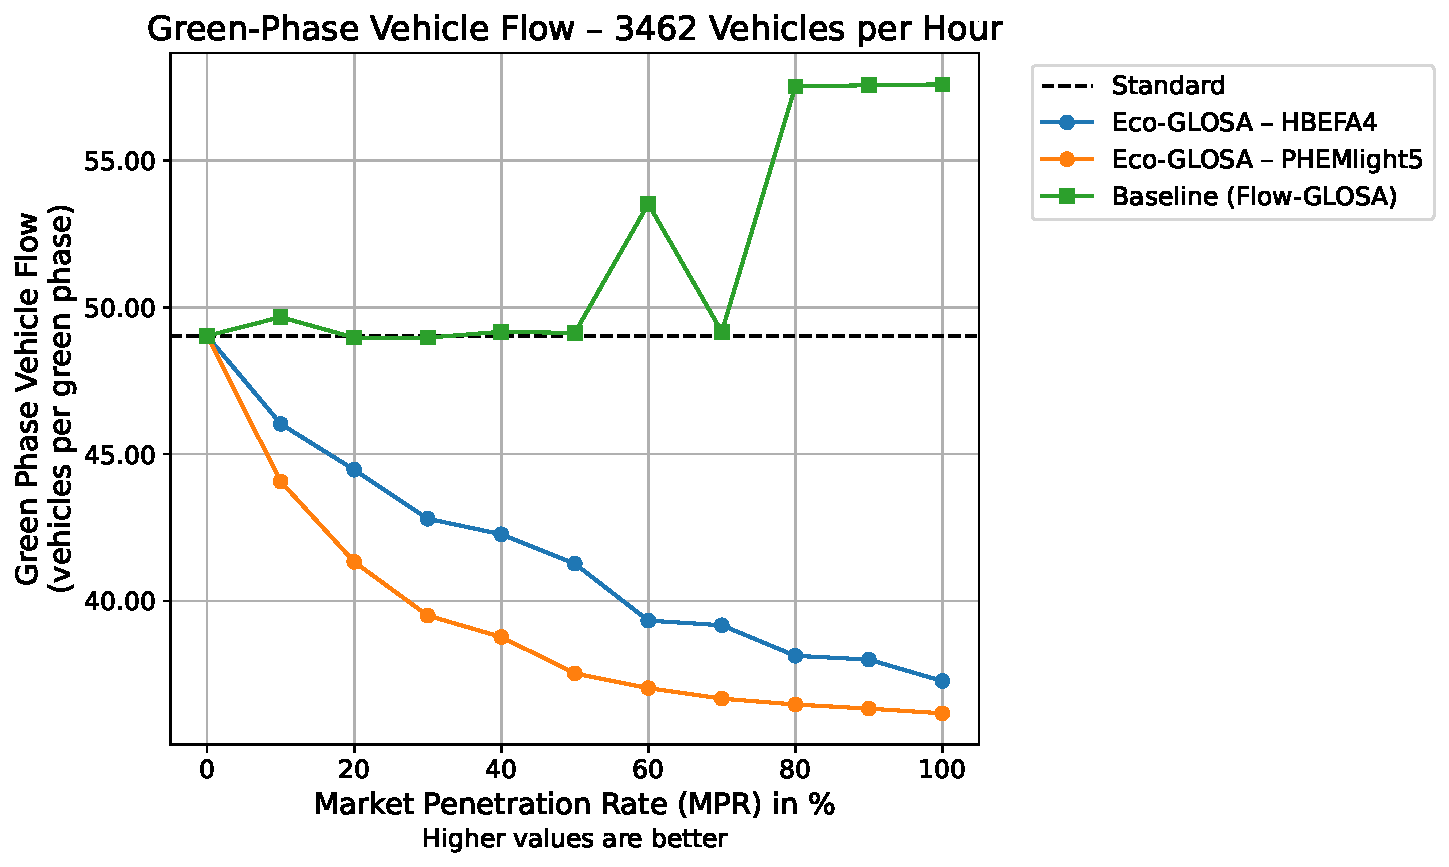
\includegraphics[width=\textwidth]{data/img/GreenPhaseVehicleFlow/GreenPhaseVehicleFlow_Cars2500.pdf}
    \caption{$3462~\unit{\veh\per\hour}$}
    \label{fig:flow_3462}
  \end{subfigure}
  \caption[]{%
    (continued) Green–phase vehicle flow as a function of \ac{mpr} for the high‐demand scenario at $3462~\unit{\veh\per\hour}$.%
  }
\end{figure}

The primary cause for this behaviour is an inherent design constraint of the \ac{eco-glosa} algorithm: it only provides speed advisories that are equal to or less than the vehicle's initial speed. At high traffic densities ($2769~\unit{\veh\per\hour}$ and above), this conservative approach systematically reduces the average speed of equipped vehicles. As the penetration rate increases, the overall platoon velocity decreases, leading to platoon compression. Consequently, the number of vehicles arriving at the intersection exceeds the capacity that can be discharged during the green phase, resulting in queue formation and the onset of congestion. In these dense traffic conditions, unequipped vehicles have limited ability to manoeuvre or bypass the slower-moving equipped vehicles, forcing them to adopt the reduced platoon speed and further contributing to the decline in throughput. This progressive speed reduction is confirmed by the average vehicle speed data presented in the following section.
\mynewline
This phenomenon is exacerbated under the PHEMlight5 emission model. PHEMlight5 assigns a higher cost penalty to even minor acceleration events. To minimise these costs, the \ac{eco-glosa} controller advises even more conservative speed profiles, which accelerates the onset of congestion at lower demand levels, as observed at $2769~\unit{\veh\per\hour}$.
Furthermore, this mechanism explains the severe, non-recoverable congestion indicated by outliers in the results of HBEFA4 at a demand of $2769~\unit{\veh\per\hour}$. When a vehicle, already slowed by incipient congestion, receives a new advisory, \ac{eco-glosa} is unable to recommend a higher speed even if conditions ahead improve. This vehicle becomes a persistent moving bottleneck, initiating a cascading failure by forcing subsequent vehicles to reduce their speed. This domino effect progressively degrades the overall traffic flow as newly arriving \ac{eco-glosa} vehicles receive increasingly lower speed advisories.
\mynewline
In contrast, the \ac{flow-glosa} controller is designed to maximise throughput and is permitted to advise acceleration. This allows it to issue higher speed advisories to slower vehicles, enabling them to catch up to the green wave and increase the vehicle discharge rate per cycle. This fundamental design difference explains why \ac{flow-glosa} can improve capacity where \ac{eco-glosa}, by design, can only maintain or reduce it.

\begin{table}[htb]
  \centering
  \caption[Green-phase vehicle throughput for all volumes and \ac{mpr} values]{Green-phase vehicle throughput, measured in vehicles per cycle, across all simulated traffic volumes and \ac{mpr} values. The Standard scenario denotes uncontrolled traffic ($0\%$ \ac{mpr}), while Baseline refers to the \ac{flow-glosa} controller.}
  \label{tab:GreenPhaseFlow}
  \resizebox{\textwidth}{!}{%
  \begin{tabular}{r l l r *{10}{r}}
    \toprule
    Vehicles & Algorithm                   & Fuel Model       & \textbf{0\% (Standard)} & 10\%  & 20\%  & 30\%  & 40\%  & 50\%  & 60\%  & 70\%  & 80\%  & 90\%  & 100\% \\
    \midrule
    69   & \ac{eco-glosa}              & HBEFA4           & \textbf{1.17} & 1.17  & 1.17  & 1.17  & 1.17  & 1.13  & 1.17  & 1.17  & 1.13  & 1.17  & 1.17  \\
    69   & Baseline (\ac{flow-glosa})  & HBEFA4           & \textbf{1.17} & 1.17  & 1.17  & 1.17  & 1.17  & 1.13  & 1.17  & 1.17  & 1.17  & 1.17  & 1.17  \\
    69   & \ac{eco-glosa}              & PHEMLIGHT5       & \textbf{1.17} & 1.17  & 1.17  & 1.17  & 1.17  & 1.13  & 1.17  & 1.17  & 1.17  & 1.17  & 1.17  \\
    69   & Baseline (\ac{flow-glosa})  & PHEMLIGHT5       & \textbf{1.17} & 1.17  & 1.17  & 1.17  & 1.17  & 1.13  & 1.17  & 1.17  & 1.17  & 1.17  & 1.17  \\
    \midrule
    138  & \ac{eco-glosa}              & HBEFA4           & \textbf{2.30} & 2.30  & 2.30  & 2.27  & 2.27  & 2.27  & 2.27  & 2.30  & 2.30  & 2.27  & 2.27  \\
    138  & Baseline (\ac{flow-glosa})  & HBEFA4           & \textbf{2.30} & 2.30  & 2.30  & 2.30  & 2.27  & 2.27  & 2.27  & 2.30  & 2.30  & 2.30  & 2.27  \\
    138  & \ac{eco-glosa}              & PHEMLIGHT5       & \textbf{2.30} & 2.30  & 2.30  & 2.27  & 2.27  & 2.27  & 2.27  & 2.30  & 2.30  & 2.30  & 2.27  \\
    138  & Baseline (\ac{flow-glosa})  & PHEMLIGHT5       & \textbf{2.30} & 2.30  & 2.30  & 2.30  & 2.27  & 2.27  & 2.27  & 2.30  & 2.30  & 2.30  & 2.27  \\
    \midrule
    346  & \ac{eco-glosa}              & HBEFA4           & \textbf{5.73} & 5.70  & 5.77  & 5.73  & 5.73  & 5.77  & 5.73  & 5.73  & 5.73  & 5.70  & 5.73  \\
    346  & Baseline (\ac{flow-glosa})  & HBEFA4           & \textbf{5.73} & 5.73  & 5.77  & 5.70  & 5.73  & 5.73  & 5.77  & 5.70  & 5.73  & 5.70  & 5.73  \\
    346  & \ac{eco-glosa}              & PHEMLIGHT5       & \textbf{5.73} & 5.73  & 5.73  & 5.70  & 5.77  & 5.73  & 5.73  & 5.70  & 5.70  & 5.70  & 5.77  \\
    346  & Baseline (\ac{flow-glosa})  & PHEMLIGHT5       & \textbf{5.73} & 5.73  & 5.77  & 5.70  & 5.73  & 5.73  & 5.77  & 5.70  & 5.73  & 5.70  & 5.73  \\
    \midrule
    692  & \ac{eco-glosa}              & HBEFA4           & \textbf{11.57} & 11.60 & 11.57 & 11.57 & 11.60 & 11.57 & 11.57 & 11.57 & 11.57 & 11.53 & 11.63 \\
    692  & Baseline (\ac{flow-glosa})  & HBEFA4           & \textbf{11.57} & 11.60 & 11.60 & 11.60 & 11.60 & 11.60 & 11.60 & 11.60 & 11.60 & 11.60 & 11.57 \\
    692  & \ac{eco-glosa}              & PHEMLIGHT5       & \textbf{11.57} & 11.57 & 11.53 & 11.53 & 11.57 & 11.57 & 11.60 & 11.57 & 11.50 & 11.53 & 11.63 \\
    692  & Baseline (\ac{flow-glosa})  & PHEMLIGHT5       & \textbf{11.57} & 11.60 & 11.60 & 11.60 & 11.60 & 11.60 & 11.60 & 11.60 & 11.60 & 11.60 & 11.57 \\
    \midrule
    1385 & \ac{eco-glosa}              & HBEFA4           & \textbf{23.03} & 22.97 & 23.07 & 22.97 & 23.03 & 23.10 & 23.03 & 23.03 & 22.97 & 23.07 & 23.03 \\
    1385 & Baseline (\ac{flow-glosa})  & HBEFA4           & \textbf{23.03} & 23.07 & 23.03 & 23.07 & 23.10 & 23.17 & 23.03 & 23.10 & 23.13 & 23.07 & 23.07 \\
    1385 & \ac{eco-glosa}              & PHEMLIGHT5       & \textbf{23.03} & 23.07 & 23.03 & 23.03 & 23.10 & 23.07 & 23.07 & 22.93 & 22.93 & 23.00 & 23.03 \\
    1385 & Baseline (\ac{flow-glosa})  & PHEMLIGHT5       & \textbf{23.03} & 23.07 & 23.03 & 23.03 & 23.10 & 23.07 & 23.07 & 22.93 & 22.93 & 23.00 & 23.03 \\
    \midrule
    2077 & \ac{eco-glosa}              & HBEFA4           & \textbf{34.63} & 34.70 & 34.67 & 34.63 & 34.67 & 34.63 & 34.70 & 34.63 & 34.63 & 34.63 & 34.67 \\
    2077 & Baseline (\ac{flow-glosa})  & HBEFA4           & \textbf{34.63} & 34.60 & 34.63 & 34.63 & 34.67 & 34.53 & 34.60 & 34.60 & 34.70 & 34.63 & 34.70 \\
    2077 & \ac{eco-glosa}              & PHEMLIGHT5       & \textbf{34.63} & 34.70 & 34.60 & 34.63 & 34.73 & 34.63 & 34.77 & 34.67 & 34.67 & 34.63 & 34.70 \\
    2077 & Baseline (\ac{flow-glosa})  & PHEMLIGHT5       & \textbf{34.63} & 34.60 & 34.63 & 34.63 & 34.67 & 34.53 & 34.60 & 34.60 & 34.70 & 34.63 & 34.70 \\
    \midrule
    2769 & \ac{eco-glosa}              & HBEFA4           & \textbf{46.03} & 46.10 & 46.03 & 41.90 & 42.67 & 46.20 & 39.30 & 46.30 & 46.07 & 46.03 & 46.03 \\
    2769 & Baseline (\ac{flow-glosa})  & HBEFA4           & \textbf{46.03} & 46.13 & 46.03 & 45.97 & 46.07 & 46.03 & 46.17 & 46.17 & 46.07 & 46.07 & 46.13 \\
    \textbf{2769} & \textbf{\ac{eco-glosa}} & \textbf{PHEMLIGHT5} & \textbf{46.03} & \textbf{44.47} & \textbf{41.73} & \textbf{39.33} & \textbf{38.37} & \textbf{37.57} & \textbf{37.17} & \textbf{36.97} & \textbf{36.67} & \textbf{35.90} & \textbf{37.83} \\
    2769 & Baseline (\ac{flow-glosa})  & PHEMLIGHT5       & \textbf{46.03} & 46.13 & 46.03 & 45.97 & 46.07 & 46.03 & 46.17 & 46.17 & 46.07 & 46.07 & 46.13 \\
    \midrule
    3462 & \ac{eco-glosa}              & HBEFA4           & \textbf{49.03} & 46.03 & 44.47 & 42.80 & 42.27 & 41.27 & 39.33 & 39.17 & 38.13 & 38.00 & 37.27 \\
    3462 & Baseline (\ac{flow-glosa})  & HBEFA4           & \textbf{49.03} & 49.67 & 48.97 & 48.97 & 49.17 & 49.13 & 53.53 & 49.17 & 57.53 & 57.57 & 57.60 \\
    3462 & \ac{eco-glosa}              & PHEMLIGHT5       & \textbf{49.03} & 44.07 & 41.33 & 39.50 & 38.77 & 37.53 & 37.03 & 36.67 & 36.47 & 36.33 & 36.17 \\
    3462 & Baseline (\ac{flow-glosa})  & PHEMLIGHT5       & \textbf{49.03} & 49.67 & 48.97 & 48.97 & 49.17 & 49.13 & 53.53 & 49.17 & 57.53 & 57.57 & 57.60 \\
    \bottomrule
  \end{tabular}%
  }
\end{table}
